\documentclass[10pt,a4paper]{article}
\usepackage[utf8]{inputenc}
\usepackage[T1]{fontenc}
\usepackage{lmodern}
\usepackage[english]{babel}
\usepackage[margin=2.0cm]{geometry}
\usepackage{amsmath,amssymb,mathtools,bm}
\usepackage{booktabs,array,tabularx}
\newcolumntype{L}[1]{>{\raggedright\arraybackslash}p{#1}}
\usepackage{graphicx}
\usepackage{float}
\usepackage[font=small]{caption}
\usepackage{xcolor}
\usepackage{tikz}
\usetikzlibrary{arrows.meta,positioning,calc,fit}
\usepackage[hidelinks]{hyperref}
\usepackage{url}
\makeatletter\g@addto@macro{\UrlBreaks}{\do\_\do/}\makeatother
\numberwithin{equation}{section}
\setlength{\emergencystretch}{3em}
\newcommand{\note}[1]{\begin{center}\fcolorbox{red!70!black}{red!5}{\parbox{0.94\linewidth}{\small\textbf{Note.} #1}}\end{center}}
\newcommand{\KppA}{7.92}
\newcommand{\KpvA}{187}
\newcommand{\KivA}{0.37}
\newcommand{\KppP}{8.02}
\newcommand{\KpvP}{54}
\newcommand{\KivP}{1.28}
\newcommand{\kpA}{14.8}
\newcommand{\kiA}{24.1}
\newcommand{\qiA}{600}
\newcommand{\qpA}{147}
\newcommand{\nOkA}{23}
\newcommand{\nScanA}{35}
\newcommand{\nRedA}{9}
\newcommand{\nFullA}{15}
\newcommand{\tauIA}{0.6}
\newcommand{\kpP}{129.4}
\newcommand{\kiP}{123.1}
\newcommand{\qiP}{\ensuremath{1.61\times10^{4}}}
\newcommand{\qpP}{\ensuremath{1.66\times10^{4}}}
\newcommand{\nOkP}{36}
\newcommand{\nScanP}{48}
\newcommand{\nRedP}{11}
\newcommand{\nFullP}{24}
\newcommand{\tauIP}{1.1}
\newcommand{\rhoMaxA}{0.99956}
\newcommand{\robModA}{0.61}
\newcommand{\iCmdA}{17.6}
\newcommand{\iCmdCA}{12.2}
\newcommand{\bwCA}{2.11}
\newcommand{\bwLA}{2.40}
\newcommand{\zOneA}{0.055}
\newcommand{\zOneCA}{0.023}
\newcommand{\rhoMaxP}{0.99989}
\newcommand{\robModP}{0.53}
\newcommand{\iCmdP}{10.0}
\newcommand{\iCmdCP}{5.9}
\newcommand{\bwCP}{2.69}
\newcommand{\bwLP}{8.02}
\newcommand{\zOneP}{0.014}
\newcommand{\zOneCP}{0.014}
\newcommand{\errCA}{1165}
\newcommand{\errLA}{951}
\newcommand{\rmsCA}{411}
\newcommand{\rmsLA}{367}
\newcommand{\rmsDA}{11}
\newcommand{\errDA}{18}
\newcommand{\tCA}{1.7}
\newcommand{\tLA}{2.1}
\newcommand{\oLA}{274}
\newcommand{\iCA}{11.6}
\newcommand{\iLA}{14.7}
\newcommand{\iDA}{27}
\newcommand{\errCP}{1125}
\newcommand{\errLP}{341}
\newcommand{\rmsCP}{447}
\newcommand{\rmsLP}{137}
\newcommand{\rmsDP}{69}
\newcommand{\errDP}{70}
\newcommand{\tCP}{1.0}
\newcommand{\tLP}{2.4}
\newcommand{\oLP}{79}
\newcommand{\iCP}{5.1}
\newcommand{\iLP}{9.5}
\newcommand{\iDP}{85}


\tikzset{
  lab/.style={font=\scriptsize, inner sep=1.5pt},
  sig/.style={-{Latex[length=2mm]}, thick},
  blk/.style={draw, rounded corners, align=center, minimum height=0.9cm, fill=blue!4, font=\small},
  sum/.style={draw, circle, inner sep=1.2pt, font=\scriptsize},
}

\title{LQG position control of the LUCY mount in the form of Gawronski:\\ PI and flexible mode controller compared with the cascade on the V2 doublets}
\author{Generated by \texttt{build\_lqg\_report.py}\\ \small\texttt{sim/gimbal\_multidof/report\_lqg\_gawronski}}
\date{\today}
\begin{document}
\maketitle

\paragraph{Purpose.} The model of the LUCY mount, with Dahl bearings and the AKD2G drive, reproduces the position of the V2 doublets in closed loop (\path{report_dahl_resampled}). This report uses that model to design a position controller in the form proposed by W.~Gawronski (\emph{Modeling and Control of Antennas and Telescopes}, Springer, 2008, Chapter~8): a PI on the estimated position error plus a flexible mode controller, with gains from an LQG synthesis. The controller is compared with the present cascade of position, velocity and current loops, on the same doublet references.

\paragraph{Main results.} All results of the LQG controller are simulations: it has not been run on the mount.
\begin{itemize}
\item \textbf{Architecture.} As in the book, the plant of the synthesis is the closed velocity loop. The current and velocity loops stay in the drive; the LQG controller replaces the position gain and runs in the master at 1\,kHz. The state is $[\hat e_i,\ \hat e,\ \hat x_f]$. Gains come from \texttt{dlqr} and \texttt{dlqe} of python-control.
\item \textbf{Following error improves.} Median over the moves, azimuth and elevation: largest error $-$\errDA\,\% and $-$\errDP\,\%, rms error $-$\rmsDA\,\% and $-$\rmsDP\,\%. The closed-loop bandwidth goes from \bwCA\ to \bwLA\,Hz in azimuth and from \bwCP\ to \bwLP\,Hz in elevation.
\item \textbf{The price is overshoot, settling and current.} Median overshoot goes from about 0 to \oLA\,mdeg in azimuth and \oLP\,mdeg in elevation, settling within $\pm5$\,mdeg from \tCA\ to \tLA\,s and from \tCP\ to \tLP\,s, and peak current rises by \iDA\,\% and \iDP\,\%. An integral action in the position loop gives zero mean error on a step, so overshoot cannot be removed on these references without a command preprocessor or feedforward.
\item \textbf{What limits the gains differs by axis.} In azimuth the current stops $k_p$ near \kpA\,s$^{-1}$. In elevation the current has margin and $k_p$ reaches \kpP\,s$^{-1}$, stopped by the stability margin with the bearings stuck; a higher $k_i$ gives a limit cycle with the friction. The elevation gains rely on a noise-free encoder and on the model of the velocity loop, so they are the least proven part of this design.
\item \textbf{Flexible modes.} In azimuth $K_f$ raises the damping of the 56\,Hz fork mode from \zOneCA\ to \zOneA, at a cost in gain margin (26 to 10\,dB). In elevation any flexible weight broke the margin constraint and was left at zero, so the damping of the modes does not change. The modes are 7 to 23 times above the bandwidth and do not appear in the doublets.
\end{itemize}

\note{The H7 configuration still contains placeholder data; the figures carry the label ``result from placeholder parameters''. $K_{pp}$, $K_{pv}$, $K_{iv}$ of the cascade are effective gains estimated on the 1$^\circ$ doublet, not the drive file values, and the LQG plant inherits $K_{pv}$, $K_{iv}$ (Section~\ref{sec:limits}).}

\tableofcontents

%% ===================================================================================================
\section{Model}\label{sec:model}
\subsection{Structure and bearings}
Each axis is the lumped modal model identified on the WorkBench frequency responses with the unweighted cost of \path{report_dahl_resampled} (uniform grid in $\ln f$, 1--150\,Hz):
\begin{equation}
\mathbf M\ddot{\mathbf x}+\mathbf C\dot{\mathbf x}+\mathbf K_0\mathbf x=\mathbf e\,\tau_m-\mathbf v\,T_b,\qquad \theta_\mathrm{enc}=\mathbf c^T\mathbf x,\qquad \delta=\mathbf v^T\mathbf x,
\end{equation}
with viscous modal damping, $\tau_m=g_{K_t}K_ti$ and the bearings as a pure Dahl element on the deflection $\delta$:
\begin{equation}
\dot z=\dot\delta-\frac{\sigma_0|\dot\delta|}{T_c}z,\qquad T_b=\sigma_0z .
\end{equation}
$T_c$ comes from the doublets and $\sigma_0$ from the frequency responses (Table~\ref{tab:structure}). The element is a spring $\sigma_0$ for small motion and Coulomb friction $T_c$ in sliding. Figures~\ref{fig:freq_el} and~\ref{fig:freq_az} show the fit in frequency.

\begin{table}[H]\centering\footnotesize
\caption{Structural model. Last two columns: lightly damped poles of the closed velocity loop; in azimuth the 65\,Hz pole belongs to the resonator of the drive, the others are structural modes.}\label{tab:structure}
\begin{tabular}{lrrrrll}\toprule
axis & $\sigma_0$ [N\,m/rad] & $T_c$ [N\,m] & $g_{K_t}$ & $\tau_d$ [ms] & lightly damped poles [Hz] & damping \\ \midrule
azimuth & 1571 & 0.232 & 0.900 & 0.48 & 56.0 / 65.1 & 0.023 / 0.028 \\
elevation & 17837 & 0.407 & 1.051 & 0.47 & 56.1 / 98.3 & 0.014 / 0.031
\\ \bottomrule
\end{tabular}\end{table}

\begin{figure}[H]\centering
\includegraphics[width=0.86\linewidth]{figures/freq_elevation.pdf}
\caption{Elevation plant: measurements and hybrid models from \texttt{report\_dahl\_resampled}. The model used here is ``uniform in $\ln f$''.}\label{fig:freq_el}
\end{figure}
\begin{figure}[H]\centering
\includegraphics[width=0.86\linewidth]{figures/freq_azimuth.pdf}
\caption{Azimuth plant: as Figure~\ref{fig:freq_el}.}\label{fig:freq_az}
\end{figure}

\subsection{Drive and motor}\label{sec:drive}
The drive is the AKD2G model of \path{closedLoopModel/lucy_cl}:
\begin{gather}
v_\mathrm{cmd}=K_{pp}(p_\mathrm{cmd}-\theta_\mathrm{enc}),\qquad
i_\mathrm{cmd}=K_{pv}\Bigl(1+\frac{2\pi K_{iv}}{s}\Bigr)H_\mathrm{fwd}(s)\bigl(v_\mathrm{cmd}-H_\mathrm{fb}(s)\dot\theta_\mathrm{enc}\bigr),\label{eq:cascade}\\
u=K_{pi}\Bigl(1+\frac{R}{Ls}\Bigr)(i_\mathrm{cmd}-i),\qquad L_\mathrm{ph}\frac{di}{dt}=\frac u2-R_\mathrm{ph}i-K_{e,\mathrm{ph}}\omega_r .
\end{gather}
Filters and current gain come from the WorkBench exports of the V2 session (Table~\ref{tab:drive}), the motor from the TBM(S)-7646-A datasheet. $K_{pp}$, $K_{pv}$, $K_{iv}$ are effective gains estimated on the following error of the 1$^\circ$ doublet: the values of the drive files do not reproduce the doublets, which are run by the PLC. Without feedforward, the following error at velocity $v$ is $v/K_{pp}$, about 1.3$^\circ$ at 10$^\circ$/s.

\begin{table}[H]\centering\footnotesize\setlength{\tabcolsep}{3pt}
\caption{Drive: effective gains of the cascade, current-loop bandwidth, current limit, and active filters. $K_{pp}$ [1/s], $K_{pv}$ [A\,s/rad], $K_{iv}$ [Hz].}\label{tab:drive}
\begin{tabular}{lrrrrrL{4.4cm}L{3.6cm}}\toprule
axis & $K_{pp}$ & $K_{pv}$ & $K_{iv}$ & $f_i$ [Hz] & $i_\mathrm{max}$ [A] & $H_\mathrm{fwd}$ & $H_\mathrm{fb}$ \\ \midrule
azimuth & 7.92 & 187.4 & 0.37 & 1509 & 18 & resonator 65 Hz, G = +10.0 dB, Q = 10; num 500 Hz/Q 3, den 14 Hz/Q 3 & none \\
elevation & 8.02 & 53.5 & 1.28 & 1509 & 18 & resonator 50 Hz, G = -12.0 dB, Q = 6; resonator 96 Hz, G = -12.0 dB, Q = 6 & num 5000 Hz/Q 0.707107, den 800 Hz/Q 0.707107; num 5000 Hz/Q 0.707107, den 800 Hz/Q 0.707107; low pass 200 Hz (observer)
\\ \bottomrule
\end{tabular}\end{table}

\subsection{Simulation}\label{sec:sim}
Structure, motor and drive are linear below the limits of the drive. They are discretised exactly with step 0.1\,ms, with the Dahl state advanced exactly over each step at the mean bearing velocity. The initial state is the equilibrium with the friction holding the measured holding current, limited to $T_c$. After each run the current command, the velocity integrator and the phase voltage are checked against the limits. The cascade is the same simulation as in \path{report_dahl_resampled}.

%% ===================================================================================================
\section{Controller}\label{sec:ctrl}
\subsection{Architecture}
Gawronski (Figures~8.1 and~8.4, Section~1.2) treats the antenna as two loops: the velocity loop, closed by the drive, and the position loop, closed by the computer. The LQG controller replaces the PI of the position loop and sends a velocity command to the velocity loop. The same is done here (Figure~\ref{fig:arch}). The drive keeps \eqref{eq:cascade} with $K_{pp}=0$ and its velocity input driven by $u$; $K_{pv}$, $K_{iv}$ and the filters are the same as in the cascade, so the comparison concerns the position loop alone. Gawronski calls this configuration PL (Table~8.3).

\begin{figure}[H]\centering
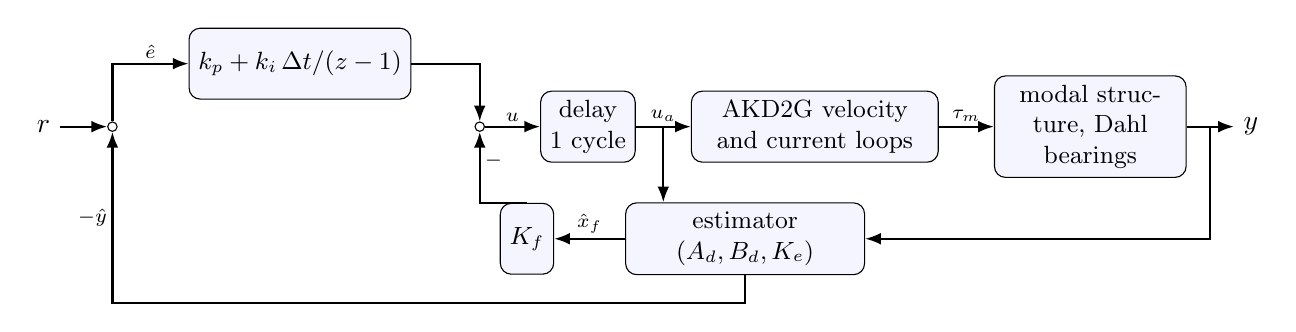
\begin{tikzpicture}[node distance=7mm]
\node (r) {$r$};
\node[sum, right=6mm of r] (s) {};
\node[blk, right=9mm of s, yshift=8mm] (pi) {$k_p+k_i\,\Delta t/(z-1)$};
\node[sum, right=8mm of pi, yshift=-8mm] (s2) {};
\node[blk, right=7mm of s2] (d) {delay\\ 1 cycle};
\node[blk, right=7mm of d, text width=2.9cm] (vl) {AKD2G velocity and current loops};
\node[blk, right=7mm of vl, text width=2.2cm] (pl) {modal structure, Dahl bearings};
\node[right=6mm of pl] (y) {$y$};
\node[blk, below=9mm of s2, xshift=6mm] (kf) {$K_f$};
\node[blk, right=9mm of kf, text width=2.8cm] (est) {estimator $(A_d,B_d,K_e)$};
\draw[sig] (r) -- (s); \draw[sig] (s) |- node[pos=0.75, above, lab]{$\hat e$} (pi.west);
\draw[sig] (pi.east) -| (s2.north); \draw[sig] (s2) -- node[above, lab]{$u$} (d); \draw[sig] (d) -- node[above, lab]{$u_a$} (vl); \draw[sig] (vl) -- node[above, lab]{$\tau_m$} (pl); \draw[sig] (pl) -- (y);
\draw[sig] (kf.north) -| node[pos=0.8, right, lab]{$-$} (s2.south);
\draw[sig] (est.west) -- node[above, lab]{$\hat x_f$} (kf.east);
\draw[sig] ($(pl.east)!0.5!(y.west)$) |- (est.east);
\coordinate (mu) at ($(d.east)!0.5!(vl.west)$); \draw[sig] (mu) -- (mu |- est.north);
\draw[sig] (est.south) -- ++(0,-0.35) -| node[pos=0.75, left, lab]{$-\hat y$} (s.south);
\end{tikzpicture}
\caption{LQG position loop. PI on the estimated error and flexible mode controller run in the master at $\Delta t=1$\,ms; the velocity and current loops stay in the drive.}\label{fig:arch}
\end{figure}

\subsection{Synthesis model}
\paragraph{Velocity loop.} With friction removed (in sliding it is a disturbance), the structure, motor and drive give the plant from $u$ to the encoder,
\begin{equation}
\dot{\mathbf x}=\mathbf A\mathbf x+\mathbf Bu,\qquad y=\mathbf C\mathbf x ,
\end{equation}
of order \nFullA\ in azimuth and \nFullP\ in elevation. Its rigid pole is at the origin with residue close to 1. In elevation the residue is 0.993, because a 0.15\,Hz stiffness in the model makes the DC gain of the velocity loop finite (about 146).

\paragraph{Modal form and truncation} (book 2.23--2.32, 4.4--4.12). The plant is transformed to real block-modal form and each mode gets its $H_\infty$ norm, the height of its peak. The rigid mode is always kept. The others are kept if they lie within the validated band ($f\leq150$\,Hz) and have $\|G_i\|_\infty\geq10^{-5}$ (Tables~\ref{tab:modes_az} and~\ref{tab:modes_el}), giving order \nRedA\ and \nRedP. The states of a mode are scaled so that its input and output norms are equal, which makes the weights comparable. Besides the structural modes, the set contains the poles of the velocity loop and of the drive filters: in the book they all belong to the velocity loop that is identified as the plant. Figures~\ref{fig:vl_az} and~\ref{fig:vl_el} compare the full and reduced models.

\begin{table}[H]\centering\footnotesize
\begin{minipage}{0.48\linewidth}\centering
\caption{Azimuth: poles of the velocity loop.}\label{tab:modes_az}
\begin{tabular}{rrrrl}\toprule
$f$ [Hz] & $\zeta$ & $\|G\|_\infty$ [s] & states & kept \\ \midrule
rigid & -- & $\infty$ & 1 & yes \\
0.43 & -- & 0.0802 & 1 & yes \\
2.60 & -- & 0.0812 & 1 & yes \\
13.37 & 0.209 & \ensuremath{3.83\times10^{-3}} & 2 & yes \\
55.98 & 0.023 & \ensuremath{6.84\times10^{-4}} & 2 & yes \\
65.11 & 0.028 & \ensuremath{1.42\times10^{-4}} & 2 & yes \\
97.80 & -- & \ensuremath{1.89\times10^{-8}} & 1 &  \\
951.84 & 0.004 & \ensuremath{1.97\times10^{-4}} & 2 &  \\
1500.47 & -- & \ensuremath{4.18\times10^{-7}} & 1 &  \\
2259.34 & 0.050 & \ensuremath{2.55\times10^{-6}} & 2 & 
\\ \bottomrule
\end{tabular}
\end{minipage}\hfill
\begin{minipage}{0.48\linewidth}\centering
\caption{Elevation: poles of the velocity loop.}\label{tab:modes_el}
\begin{tabular}{rrrrl}\toprule
$f$ [Hz] & $\zeta$ & $\|G\|_\infty$ [s] & states & kept \\ \midrule
rigid & -- & $\infty$ & 1 & yes \\
1.86 & 0.706 & 0.0886 & 2 & yes \\
49.42 & 0.168 & \ensuremath{2.22\times10^{-4}} & 2 & yes \\
56.12 & 0.014 & \ensuremath{1.34\times10^{-3}} & 2 & yes \\
96.38 & 0.171 & \ensuremath{6.28\times10^{-5}} & 2 & yes \\
97.81 & -- & \ensuremath{2.56\times10^{-8}} & 1 &  \\
98.25 & 0.031 & \ensuremath{6.39\times10^{-5}} & 2 & yes \\
194.60 & -- & \ensuremath{3.56\times10^{-7}} & 1 &  \\
472.41 & 0.001 & \ensuremath{4.49\times10^{-4}} & 2 &  \\
795.79 & 0.718 & \ensuremath{5.03\times10^{-9}} & 2 &  \\
804.79 & 0.697 & \ensuremath{4.49\times10^{-9}} & 2 &  \\
1215.41 & 0.001 & \ensuremath{5.48\times10^{-5}} & 2 &  \\
1507.46 & -- & \ensuremath{3.91\times10^{-8}} & 1 &  \\
10971.88 & 0.000 & \ensuremath{1.12\times10^{-8}} & 2 & 
\\ \bottomrule
\end{tabular}
\end{minipage}
\end{table}

\begin{figure}[H]\centering
\includegraphics[width=0.8\linewidth]{figures/vl_azimuth.pdf}
\caption{Azimuth: velocity loop from velocity command to encoder, full and reduced model.}\label{fig:vl_az}
\end{figure}
\begin{figure}[H]\centering
\includegraphics[width=0.8\linewidth]{figures/vl_elevation.pdf}
\caption{Elevation: as Figure~\ref{fig:vl_az}.}\label{fig:vl_el}
\end{figure}

\paragraph{State space of Gawronski} (6.1--6.7, 8.11--8.12). The position becomes the first state, and the integral of the position is added. With $\mathbf x_p=[y;\ \mathbf x_f]=\mathbf P\mathbf x_m$, $\mathbf P=[\mathbf C_m;\ \mathbf 0\ \mathbf I]$, the ZOH discretisation at $\Delta t=1$\,ms gives $(\mathbf A_d,\mathbf B_d,\mathbf C_d)$, with $\mathbf C_d=[1\ \mathbf 0]$, and
\begin{equation}
\mathbf x_o=\begin{bmatrix}y_i\\ y\\ \mathbf x_f\end{bmatrix},\qquad
\mathbf A_o=\begin{bmatrix}1&\Delta t\,\mathbf C_d\\ \mathbf 0&\mathbf A_d\end{bmatrix},\qquad
\mathbf B_o=\begin{bmatrix}0\\ \mathbf B_d\end{bmatrix}.
\end{equation}

\subsection{Gains}\label{sec:gains}
\paragraph{Regulator.} With $\mathbf Q=\mathrm{diag}(q_i,q_p,\mathbf q_f)$ and $R=1$ (8.23--8.25),
\begin{equation}
J=\sum_k\bigl(\mathbf x_o^T\mathbf Q\mathbf x_o+Ru^2\bigr),\qquad \mathbf K_c=(\mathbf B_o^T\mathbf S\mathbf B_o+R)^{-1}\mathbf B_o^T\mathbf S\mathbf A_o=[k_i\ \ k_p\ \ \mathbf K_f],
\end{equation}
which is the output of \texttt{Kc = dlqr(Ao, Bo, Q, R)}. On a rigid plant $G=1/s$, $k_i=\sqrt{q_i}$ and $k_p^2=q_p+2k_i$.

\paragraph{Estimator.} The estimator gain is the output of \texttt{Ke = dlqe(Ad, I, Cd, V, W)}, with $\mathbf V=\rho_e\mathrm{diag}(q_p,\mathbf q_f)$ and $W=1$; for $\rho_e=1$ this is the choice $V=Q$ of the book (8.26). The estimator runs on $[y;\ \mathbf x_f]$, without the integral. The integral state $y_i$ is not observable from $y$, and on the augmented model \texttt{dlqe} has no solution (it fails with ``failed to find a finite solution''). This does not change the controller, because the book does not use $\hat y_i$ either: it replaces it with the integral of the error (8.12).

\paragraph{Control law} (8.12--8.15). With $u_a$ the command that reaches the drive,
\begin{gather}
\hat{\mathbf x}_{k+1}=\mathbf A_d\hat{\mathbf x}_k+\mathbf B_du_{a,k}+\mathbf K_e(y_k-\hat y_k),\\
\hat e_k=r_k-\hat y_k,\qquad \hat e_{i,k+1}=\hat e_{i,k}+\Delta t\,\hat e_k,\qquad u_k=k_i\hat e_{i,k}+k_p\hat e_k-\mathbf K_f\hat{\mathbf x}_{f,k},\qquad u_{a,k}=u_{k-1}.
\end{gather}
The delay of one cycle models the EtherCAT transfer. With the prediction form of the estimator, a measurement reaches the drive after 2\,ms. The delay is not in the synthesis model; it is in the estimator input, in the simulation and in the margins.

\paragraph{python-control.} The synthesis uses \texttt{control.c2d}, \texttt{control.dlqr} and \texttt{control.dlqe} of python-control 0.10.2 (NumPy 2.5, SciPy 1.18), so no Riccati solver was written. Slycot is not installed; both functions then use SciPy. \texttt{dlqr} follows the MATLAB definition of the cost and the gain, and \texttt{dlqe} returns the gain of the prediction form $\mathbf A-\mathbf L\mathbf C$. Modal form and truncation are written in \path{closedLoopModel/lucy_cl/lqg.py}, because the library does not provide the block form with norms used in the book. The module has unit tests, among them one that compares the transfer function of the controller with its time-domain implementation.

%% ===================================================================================================
\section{Tuning}\label{sec:tuning}
The tuning follows the steps of Section~8.2 of the book, with the index (8.27) reduced to the doublets:
\begin{equation}
f=\frac13\sum_{\text{moves}}\Bigl(\frac{e_\mathrm{rms}}{e_\mathrm{rms,cascade}}+\frac{t_s}{1\,\mathrm{s}}+\frac{o}{0.1\,\mathrm{stroke}}\Bigr)\Big/3 ,
\end{equation}
on the 12.5\,s windows of three moves (0.1$^\circ$ \#1, 1$^\circ$ \#1, 5$^\circ$ \#2). Here $t_s$ is the settling time within $\pm5$\,mdeg after the end of the command, capped by the window, and $o$ the overshoot. The three terms have equal weight: this is a design choice, and other weights would move the result along the trade-off of Section~\ref{sec:res}. The constraints are:
\begin{itemize}
\item $k_i\leq0.25k_p^2$, the critical integral gain (7.9);
\item peak current at most 15\,A on the three moves (limit 18\,A; the book limits $q_p$ by the available acceleration);
\item $|1+L|\geq0.5$ with the velocity-loop model with bearings sliding, with bearings stuck ($\sigma_0$), and with the measured frequency response (1--150\,Hz);
\item stable closed-loop poles with the full-order plant, bearings sliding and stuck.
\end{itemize}

\paragraph{Steps 1--3: $q_p$ and $q_i$.} With zero flexible weights, $k_p$ and $k_i/(0.25k_p^2)$ are scanned on a grid, and the weights are computed with the rigid relations (Figure~\ref{fig:scan}); \nOkA\ of \nScanA\ candidates meet the constraints in azimuth and \nOkP\ of \nScanP\ in elevation. The two axes stop for different reasons:
\begin{itemize}
\item \textbf{Azimuth: current.} The best admissible candidate has $k_p=\kpA$\,s$^{-1}$, $k_i=\kiA$\,s$^{-2}$. Higher $k_p$ and $k_i$ give a lower index but exceed 15\,A (Figure~\ref{fig:scan}).
\item \textbf{Elevation: margin with stuck bearings and limit cycle.} The current has margin (9.9\,A), and $k_p$ grows until $|1+L|$ with the bearings stuck reaches the minimum 0.5, near $k_p=155$\,s$^{-1}$. The regulator moves the 1.9\,Hz poles of the velocity loop to 7.4\,Hz (Table~\ref{tab:poles}), so that $k_p$ acts beyond the velocity-loop bandwidth. $k_i$ is limited separately. At every $k_p$ of the grid, the fraction 0.1 of the critical gain violates the margin, with the minimum below 0.1\,Hz with the bearings stuck. In the time domain, at $k_p\approx18$, the position integrator gives a limit cycle with the friction: at $k_i\approx28$ the axis moves for 94\,\% of the window after the command, and at $k_i\approx80$ the residual error reaches $\pm53$\,mdeg at 0.1$^\circ$ (Table~\ref{tab:hunting}). The final design has $k_p/k_i\approx\tauIP$\,s (\tauIA\,s in azimuth). At 0.1$^\circ$ it still creeps for 67\,\% of the window after the command, with a residual error of at most 3\,mdeg in the last 3\,s.
\end{itemize}

\paragraph{Step 4: flexible weights.} The weights of the structural modes and $\rho_e$ are scanned, and the design with the highest damping is kept if it meets the constraints and worsens the index by at most 5\,\% (Tables~\ref{tab:flex_az} and~\ref{tab:flex_el}). In azimuth this selects $q_f=3\times10^4$. In elevation, already at $q_f=10^3$ the margin falls below the constraint (0.49) and the index grows by over 80\,\%, so $q_f=0$ is kept; with zero weights $\mathbf K_f$ is not zero but does not change the modes. The elevation modes pass through the two $-12$\,dB resonators of the velocity path, which reduce the authority of the velocity command.

The first choice of the book, $V=Q$ ($\rho_e=1$), is not always adequate here. With small $q_f$ the estimator weight $\rho_e$ has little effect, but in azimuth at $q_f=3\times10^4$ the value $\rho_e=1$ gives $|1+L|=0.02$, and $\rho_e=10^{-3}$ gives 0.63. The encoder is noise-free in these simulations, so this scan does not test the choice of $\rho_e$ against noise.

\begin{figure}[H]\centering
\includegraphics[width=0.9\linewidth]{figures/scan.pdf}
\caption{Index against $k_p$ for four integral fractions, zero flexible weights. Markers: constraints met.}\label{fig:scan}
\end{figure}

\begin{table}[H]\centering\footnotesize
\caption{Limit cycle check: 0.1$^\circ$ doublet, move \#1, $k_p\approx18$ with increasing $k_i$, and the final design. After the end of the command: largest error in the last 3\,s, time in motion, sign changes of the error; lowest $|1+L|$ with the bearings stuck.}\label{tab:hunting}
\begin{tabular}{llrrrrrr}\toprule
axis & & $k_p$ & $k_i$ & $|e|_\mathrm{max}$ [mdeg] & in motion [\%] & sign changes & $\min|1+L|$ \\ \midrule
azimuth &  & 18.0 & 2.4 & 0.2 & 5 & 1 & 0.82 \\
 &  & 18.2 & 8.0 & 0.6 & 44 & 2 & 0.81 \\
 &  & 19.0 & 28.1 & 0.2 & 50 & 4 & 0.80 \\
 &  & 21.2 & 80.4 & 0.0 & 43 & 6 & 0.78 \\
 & \textbf{final} & 14.8 & 24.1 & 0.2 & 48 & 4 & 0.63 \\
elevation &  & 17.9 & 2.4 & 1.2 & 34 & 2 & 0.70 \\
 &  & 18.1 & 8.0 & 6.2 & 47 & 3 & 0.44 \\
 &  & 18.8 & 28.1 & 23.2 & 94 & 8 & 0.30 \\
 &  & 20.7 & 80.3 & 52.9 & 98 & 16 & 0.28 \\
 & \textbf{final} & 129.4 & 123.1 & 3.1 & 67 & 4 & 0.53
\\ \bottomrule
\end{tabular}\end{table}

\begin{table}[H]\centering\footnotesize
\begin{minipage}{0.48\linewidth}\centering\setlength{\tabcolsep}{3pt}
\caption{Azimuth: flexible weights ($k_p$, $k_i$ fixed). $\zeta$: 56\,Hz mode in closed loop. Selected in bold.}\label{tab:flex_az}
\begin{tabular}{rrrrrrl}\toprule
$q_f$ & $\rho_e$ & $\|K_{f}\|$ & $\zeta$ & $|1+L|$ & $f$ & ok \\ \midrule
0 & 1.00 & 1 & 0.023 & 0.77 & 1.32 & yes \\
0 & \ensuremath{1.00\times10^{-3}} & 1 & 0.023 & 0.76 & 1.33 & yes \\
1000 & 1.00 & 9 & 0.025 & 0.76 & 1.32 & yes \\
1000 & \ensuremath{1.00\times10^{-3}} & 9 & 0.025 & 0.77 & 1.33 & yes \\
3000 & 1.00 & 25 & 0.028 & 0.74 & 1.32 & yes \\
3000 & \ensuremath{1.00\times10^{-3}} & 25 & 0.028 & 0.79 & 1.33 & yes \\
\ensuremath{1.00\times10^{4}} & 1.00 & 69 & 0.037 & 0.55 & 1.57 & yes \\
\ensuremath{1.00\times10^{4}} & \ensuremath{1.00\times10^{-3}} & 69 & 0.037 & 0.80 & 1.33 & yes \\
\ensuremath{3.00\times10^{4}} & 1.00 & 156 & 0.055 & 0.02 & 3.18 & no \\
\textbf{\ensuremath{3.00\times10^{4}}} & \textbf{\ensuremath{1.00\times10^{-3}}} & \textbf{156} & \textbf{0.055} & \textbf{0.63} & \textbf{1.33} & \textbf{yes}
\\ \bottomrule
\end{tabular}
\end{minipage}\hfill
\begin{minipage}{0.5\linewidth}\centering\setlength{\tabcolsep}{1.5pt}
\caption{Elevation: as Table~\ref{tab:flex_az}. $\zeta$: 56 and 98\,Hz modes.}\label{tab:flex_el}
\begin{tabular}{rrrrrrl}\toprule
$q_f$ & $\rho_e$ & $\|K_{f}\|$ & $\zeta$ & $|1+L|$ & $f$ & ok \\ \midrule
\textbf{0} & \textbf{1.00} & \textbf{39} & \textbf{0.014 / 0.031} & \textbf{0.53} & \textbf{1.07} & \textbf{yes} \\
0 & \ensuremath{1.00\times10^{-3}} & 39 & 0.014 / 0.031 & 0.53 & 1.07 & yes \\
1000 & 1.00 & 52 & 0.020 / 0.032 & 0.49 & 1.96 & no \\
1000 & \ensuremath{1.00\times10^{-3}} & 52 & 0.020 / 0.032 & 0.50 & 1.96 & no \\
3000 & 1.00 & 75 & 0.028 / 0.032 & 0.44 & 2.44 & no \\
3000 & \ensuremath{1.00\times10^{-3}} & 75 & 0.028 / 0.032 & 0.44 & 2.44 & no \\
\ensuremath{1.00\times10^{4}} & 1.00 & 131 & 0.046 / 0.036 & 0.37 & 2.67 & no \\
\ensuremath{1.00\times10^{4}} & \ensuremath{1.00\times10^{-3}} & 131 & 0.046 / 0.036 & 0.37 & 2.67 & no \\
\ensuremath{3.00\times10^{4}} & 1.00 & 223 & 0.077 / 0.043 & 0.32 & 2.96 & no \\
\ensuremath{3.00\times10^{4}} & \ensuremath{1.00\times10^{-3}} & 223 & 0.077 / 0.043 & 0.32 & 2.96 & no
\\ \bottomrule
\end{tabular}
\end{minipage}
\end{table}

\begin{table}[H]\centering\footnotesize\setlength{\tabcolsep}{4pt}
\caption{Final weights and gains. $k_p$ [1/s], $k_i$ [1/s$^2$]; $K_{pp}$ of the cascade for comparison.}\label{tab:weights}
\begin{tabular}{lrrrrrrrrr}\toprule
axis & $q_i$ & $q_p$ & $q_f$ & $\rho_e$ & $k_p$ & $k_i$ & $0.25k_p^2$ & $K_{pp}$ & $\|\mathbf K_f\|$ \\ \midrule
azimuth & 600 & 147 & \ensuremath{3.00\times10^{4}} & \ensuremath{1.00\times10^{-3}} & 14.75 & 24.07 & 54 & 7.92 & 156 \\
elevation & \ensuremath{1.61\times10^{4}} & \ensuremath{1.66\times10^{4}} & 0 & 1.00 & 129.35 & 123.11 & 4183 & 8.02 & 41
\\ \bottomrule
\end{tabular}\end{table}

\begin{table}[H]\centering\footnotesize
\caption{Poles of regulator and estimator (synthesis model): frequency in Hz, damping in brackets if below 1.}\label{tab:poles}
\begin{tabular}{lL{7.1cm}L{7.1cm}}\toprule
axis & regulator & estimator \\ \midrule
azimuth & 0.33; 0.36; 2.42 (0.88); 13.37 (0.21); 56.05 (0.06); 65.11 (0.03) & 0.43; 2.60; 13.37 (0.21); 59.93; 65.11 (0.03); 68.07 (0.41) \\
elevation & 0.16; 1.28; 7.42 (0.70); 49.42 (0.17); 56.12 (0.01); 96.38 (0.17); 98.25 (0.03) & 1.86 (0.71); 49.42 (0.17); 56.12 (0.01); 96.38 (0.17); 98.25 (0.03); 1547.00
\\ \bottomrule
\end{tabular}\end{table}

%% ===================================================================================================
\section{Results}\label{sec:res}
\subsection{Linear analysis}
Table~\ref{tab:linear} and Figures~\ref{fig:tf} and~\ref{fig:loop} compare the two position loops on the same velocity loop.
\begin{itemize}
\item \textbf{Bandwidth.} It grows by about 14\,\% in azimuth, where the current limits $k_p$ to about 2 times $K_{pp}$, and by a factor 3 in elevation, with $k_p$ about 16 times $K_{pp}$. In a cascade the bandwidth of the position loop depends on that of the velocity loop (book, 8.28--8.29). The state feedback on the estimated velocity-loop poles is what lets the elevation go beyond it.
\item \textbf{Disturbance rejection.} The torque response improves by 1\,dB in azimuth and 9\,dB in elevation at 1\,Hz, and more below it, with the integral action.
\item \textbf{Margins.} $|1+L|$ stays at or above 0.53 with sliding, stuck and measured plants; the lowest gain and phase margins are lower than those of the cascade on both axes (Table~\ref{tab:linear}). With $g_{K_t}\pm10\,\%$ the closed loop stays stable, with $|1+L|$ at or above \robModA\ in azimuth and \robModP\ in elevation.
\item \textbf{Measured plant.} Figure~\ref{fig:loop} replaces the model with the measured frequency response in the position loop. Below about 3\,Hz the measured loop gain is lower than the model's, since the tests are at small amplitude with the bearings near pre-sliding. The margins are confirmed in the measured band of 1--150\,Hz only, at the amplitude of those tests.
\item \textbf{Azimuth mode.} With $\mathbf K_f$ the loop gain exceeds 0\,dB by 2--4\,dB near 56\,Hz, so that the mode is phase-stabilised, where the cascade has about 45\,dB of attenuation. The gain margin falls from 26 to 10\,dB. This relies on the frequency of the mode, and the design should be checked in other poses before being used.
\end{itemize}

\begin{table}[H]\centering\footnotesize\setlength{\tabcolsep}{3pt}
\caption{Linear comparison. Bandwidth and peak of $T_{ry}$, $T_{wy}$ at 1\,Hz, lowest $|1+L|$ per plant, lowest gain and phase margins over the plants, and damping of the structural modes in the fit band.}\label{tab:linear}
\begin{tabular}{llrrrrrrrrl}\toprule
& & BW & peak & $T_{wy}$ & \multicolumn{3}{c}{$\min|1+L|$} & GM & PM & \\
\cmidrule(lr){6-8}
axis & loop & [Hz] & [dB] & [dB] & sliding & stuck & measured & [dB] & [$^\circ$] & $\zeta$ \\ \midrule
azimuth & cascade & 2.11 & -0.00 & -51.5 & 0.75 & 0.87 & 0.89 & 25.3 & 64 & 0.023 \\
 & \textbf{LQG} & 2.40 & 1.24 & -52.5 & 0.68 & 0.63 & 0.68 & 9.9 & 58 & 0.055 \\
elevation & cascade & 2.69 & -0.00 & -46.3 & 0.67 & 0.96 & 0.85 & 32.8 & 62 & 0.014 / 0.031 \\
 & \textbf{LQG} & 8.02 & 0.26 & -55.3 & 0.72 & 0.53 & 0.82 & 10.9 & 32 & 0.014 / 0.031
\\ \bottomrule
\end{tabular}\end{table}

\begin{figure}[H]\centering
\includegraphics[width=0.92\linewidth]{figures/tf.pdf}
\caption{Closed-loop transfer functions from command and from bearing torque to the encoder, bearings sliding.}\label{fig:tf}
\end{figure}
\begin{figure}[H]\centering
\includegraphics[width=0.92\linewidth]{figures/loop.pdf}
\caption{Position loop opened at the encoder: LQG with model and measured plant, cascade with measured plant.}\label{fig:loop}
\end{figure}

\subsection{Doublets}
Both schemes get the measured position reference of the 36 moves of the V2 doublets, with the same plant and velocity loop. Only the cascade was run on the real axis; the ``measured'' columns show how far the model is from the measurement, not a test of the LQG controller. In azimuth the first move of the 8$^\circ$ doublet is excluded: its window is cut by the detection of the moves. No limit is reached: the largest current command is \iCmdA\,A in azimuth (cascade \iCmdCA\,A), in that excluded window, and \iCmdP\,A in elevation (cascade \iCmdCP\,A).

\begin{table}[H]\centering\footnotesize\setlength{\tabcolsep}{4pt}
\caption{Median over the moves. Largest and rms error during the move (to 1\,s after the end of the command), overshoot, settling within $\pm5$\,mdeg after the end of the command, largest and rms current.}\label{tab:med}
\begin{tabular}{llrrrrrr}\toprule
axis & scheme & $e_\mathrm{max}$ [mdeg] & $e_\mathrm{rms}$ [mdeg] & $o$ [mdeg] & $t_s$ [s] & $i_\mathrm{max}$ [A] & $i_\mathrm{rms}$ [A] \\ \midrule
azimuth & measured (cascade, real axis) & 1144 & 408 & 4 & 0.4 & 9.9 & 3.47 \\
 & model, cascade & 1165 & 411 & 0 & 1.7 & 11.6 & 3.43 \\
 & \textbf{model, LQG} & 951 & 367 & 274 & 2.1 & 14.7 & 3.97 \\
elevation & measured (cascade, real axis) & 1269 & 482 & 0 & 1.3 & 5.5 & 1.88 \\
 & model, cascade & 1125 & 447 & 0 & 1.0 & 5.1 & 2.06 \\
 & \textbf{model, LQG} & 341 & 137 & 79 & 2.4 & 9.5 & 2.39
\\ \bottomrule
\end{tabular}\end{table}

\begin{table}[H]\centering\scriptsize\setlength{\tabcolsep}{2.6pt}
\caption{Azimuth, median of the moves of each doublet: m, measured; c, cascade on the model; L, LQG on the model.}\label{tab:db_az}
\begin{tabular}{lrrrrrrrrrrrrrrr}\toprule
& \multicolumn{3}{c}{$e_\mathrm{max}$ [mdeg]} & \multicolumn{3}{c}{$e_\mathrm{rms}$ [mdeg]} & \multicolumn{3}{c}{$o$ [mdeg]} & \multicolumn{3}{c}{$t_s$ [s]} & \multicolumn{3}{c}{$i_\mathrm{max}$ [A]} \\
\cmidrule(lr){2-4}\cmidrule(lr){5-7}\cmidrule(lr){8-10}\cmidrule(lr){11-13}\cmidrule(lr){14-16}
ampl. [$^\circ$] & m & c & L & m & c & L & m & c & L & m & c & L & m & c & L \\ \midrule
0.1 & 96 & 95 & 92 & 29 & 30 & 27 & 6 & 0 & 15 & 0.3 & 0.8 & 1.9 & 4.6 & 3.4 & 4.8 \\
0.5 & 410 & 421 & 391 & 128 & 132 & 121 & 17 & 0 & 72 & 0.4 & 1.7 & 1.5 & 9.3 & 7.9 & 10.9 \\
1 & 721 & 757 & 680 & 238 & 244 & 222 & 10 & 6 & 135 & 0.4 & 0.3 & 1.6 & 10.1 & 11.0 & 14.5 \\
3 & 1294 & 1283 & 992 & 523 & 522 & 455 & 0 & 19 & 399 & 0.4 & 2.5 & 2.2 & 10.3 & 11.6 & 14.9 \\
5 & 1296 & 1282 & 992 & 670 & 653 & 536 & 0 & 0 & 583 & 0.4 & 2.6 & 2.4 & 10.4 & 11.6 & 14.9 \\
8 & 1296 & 1283 & 992 & 889 & 857 & 544 & 0 & 0 & 834 & 0.4 & 2.2 & 2.6 & 10.0 & 11.6 & 14.9
\\ \bottomrule
\end{tabular}\end{table}

\begin{table}[H]\centering\scriptsize\setlength{\tabcolsep}{2.6pt}
\caption{Elevation: as Table~\ref{tab:db_az}.}\label{tab:db_el}
\begin{tabular}{lrrrrrrrrrrrrrrr}\toprule
& \multicolumn{3}{c}{$e_\mathrm{max}$ [mdeg]} & \multicolumn{3}{c}{$e_\mathrm{rms}$ [mdeg]} & \multicolumn{3}{c}{$o$ [mdeg]} & \multicolumn{3}{c}{$t_s$ [s]} & \multicolumn{3}{c}{$i_\mathrm{max}$ [A]} \\
\cmidrule(lr){2-4}\cmidrule(lr){5-7}\cmidrule(lr){8-10}\cmidrule(lr){11-13}\cmidrule(lr){14-16}
ampl. [$^\circ$] & m & c & L & m & c & L & m & c & L & m & c & L & m & c & L \\ \midrule
0.1 & 100 & 99 & 84 & 46 & 69 & 29 & 1 & 0 & 14 & 1.4 & 0.9 & 1.8 & 1.8 & 1.6 & 3.7 \\
0.5 & 450 & 439 & 227 & 138 & 136 & 52 & 3 & 0 & 23 & 0.2 & 2.6 & 1.4 & 4.0 & 3.6 & 8.7 \\
1 & 837 & 822 & 358 & 264 & 265 & 95 & 0 & 0 & 33 & 1.2 & 1.8 & 1.4 & 5.8 & 4.9 & 9.8 \\
3 & 1298 & 1283 & 380 & 546 & 523 & 155 & 1 & 0 & 100 & 1.2 & 1.1 & 2.7 & 5.7 & 5.8 & 9.9 \\
5 & 1314 & 1297 & 385 & 691 & 648 & 174 & 0 & 0 & 140 & 1.3 & 1.0 & 3.2 & 5.8 & 5.9 & 9.9 \\
8 & 1309 & 1297 & 385 & 818 & 775 & 181 & 0 & 0 & 183 & 1.3 & 1.0 & 3.6 & 5.7 & 5.9 & 9.9
\\ \bottomrule
\end{tabular}\end{table}

\begin{itemize}
\item \textbf{Following error.} Cruise error at 10$^\circ$/s falls from about 1283 to 990\,mdeg in azimuth and from about 1297 to 385\,mdeg in elevation. It does not reach zero: the 1\,s ramps are short compared with the integral time constant.
\item \textbf{Overshoot.} It grows with the stroke, up to about 830\,mdeg in azimuth and 180\,mdeg in elevation at 8$^\circ$. With $k_i>0$ the loop is of type 2: on a step $\int e\,dt=0$, so the area of the lag during the acceleration comes back as overshoot. The cascade has no position integrator and its model does not overshoot on the large moves; the median on the real axis is at most 17\,mdeg.
\item \textbf{Settling.} In azimuth it is comparable to the cascade model at large strokes, about 2\,s, and slower at 0.1 and 1$^\circ$; the measured axis settles in about 0.4\,s. In elevation it is 1.4--3.6\,s, against about 1--2.6\,s of the cascade model. The axis stops beyond the reference, sticks, and returns when the integrator overcomes the friction (Figure~\ref{fig:db_el}).
\item \textbf{Current.} The peaks grow with $k_p$, from 11.6 to 14.9\,A in azimuth and from 5.9 to 9.9\,A in elevation at large strokes. At 0.1$^\circ$ in elevation the first peak is a short spike of 3.7\,A against 1.6\,A.
\item \textbf{Flexible modes.} Neither scheme excites them visibly in the doublets. The value of $\mathbf K_f$ for the azimuth mode can be seen in $T_{wy}$ near 56\,Hz (Figure~\ref{fig:tf}), not in these tests.
\end{itemize}

\begin{figure}[H]\centering
\includegraphics[width=\linewidth]{figures/db_azimuth.pdf}
\caption{Azimuth: position, following error and motor current for one move of the 0.1, 1 and 5$^\circ$ doublets: measurement (cascade on the real axis), cascade and LQG on the model.}\label{fig:db_az}
\end{figure}
\begin{figure}[H]\centering
\includegraphics[width=\linewidth]{figures/db_elevation.pdf}
\caption{Elevation: as Figure~\ref{fig:db_az}.}\label{fig:db_el}
\end{figure}

\paragraph{Reading of the comparison.} On doublets, which are fast moves with no command shaping, the LQG controller trades lower following error for overshoot, higher current and, in azimuth at small strokes and in elevation at large strokes, longer settling. The gain is large in elevation and modest in azimuth, and it is not a uniform improvement. The doublets do not show its main expected benefit, the zero error at constant velocity. At the $\leq0.06^\circ$/s of the elevation on the sky, the cascade has $v/K_{pp}\approx7.5$\,mdeg of following error by this linear relation, while the position integral removes it with the time constant above. That tracking condition was not simulated here, and friction at such speeds needs its own check.

%% ===================================================================================================
\section{Limitations and open points}\label{sec:limits}
\begin{itemize}
\item \textbf{Simulation only.} The LQG controller has not been run on the mount. The model reproduces the position under the cascade, but its current fit is low (median 20\,\% in azimuth, 50\,\% in elevation in \path{report_dahl_resampled}), and the measured 7\,Hz current oscillation in azimuth is not reproduced. A controller that asks more current depends more on these parts of the model.
\item \textbf{Effective gains.} $K_{pv}$ and $K_{iv}$ are estimated, not the drive file values, and the role of the PLC loop is still open. The LQG plant is the velocity loop with those gains. It should be measured with the actual configuration before the design is used: the book identifies this plant directly from a test (3.2).
\item \textbf{Velocity-loop configuration.} The velocity loop is not retuned here. The book finds the largest gains with LQG in the velocity loop, with the position loop around it (configurations LP and LL, Table~8.3). With current as input, the rigid part would add a third integrator, $[e_i,\ e,\ \dot e,\ x_f]$ (\path{closedLoopModel/LQG_GAWRONSKI_AUDIT.md}, Section~3.3); that variant was not developed here.
\item \textbf{Command shaping.} No feedforward or command preprocessor is used, to keep the comparison with the present cascade. The book treats both (7.5, 11.1.1); they act on the overshoot and on the following error, and were not studied.
\item \textbf{Friction in the controller.} The estimator has no friction model, and the margin and limit cycle with the stuck bearings limit $k_p$ and $k_i$ in elevation. The disturbance state of \path{closedLoopModel/LQG_GAWRONSKI_AUDIT.md} (Section~3.5), or a lower $K_{iv}$, could relax it; neither was tried.
\item \textbf{Noise, quantisation, anti-windup.} The encoder is noise-free and not quantised, so nothing penalises the fast estimator or the high $k_p$ in elevation: this is the first check to make on that design. Limits were checked after the runs and never reached, so the controller has no anti-windup yet; a real one needs it, since the integrator is in the master and the limits are in the drive.
\item \textbf{Index.} The weights of the index are a choice. Another choice, for example one that accepts more tail or more overshoot, gives another point of the same trade-off.
\item \textbf{Other poses.} The model is linearised at one pose and the modes are from one set of tests. The phase-stabilised 56\,Hz azimuth mode is the most sensitive point.
\end{itemize}

\paragraph{Reproducibility.} From \path{sim/gimbal_multidof}:
\begin{itemize}
\item \texttt{analisi\_lqg\_gawronski.py}: tuning, evaluation and figures (\texttt{--riusa-taratura} keeps the saved tuning); results in \path{results_lqg_gawronski};
\item \path{closedLoopModel/lucy_cl/lqg.py}: synthesis; \path{closedLoopModel/tests/test_lqg.py}: tests;
\item \texttt{report\_lqg\_gawronski/build\_lqg\_report.py}: this report.
\end{itemize}

\end{document}
